%--------------------------------------------------------------------------%
%
%   QuanBit: AI-Based Interactive Quantum Algorithm Learning Platform
%   Product Specification Document
%
%   Document Version: 1.0.0
%   Status: Complete Product Specification
%
%--------------------------------------------------------------------------%

\documentclass[11pt, a4paper]{article}

%------------------------%
% Include LaTeX packages %
%------------------------%

\usepackage[top=2.5cm, left=2.5cm, bottom=2.5cm, right=2.5cm]{geometry}
\usepackage[nodisplayskipstretch]{setspace}
\setstretch{1.15}

\usepackage{amsmath}
\usepackage{amsfonts}
\usepackage{amssymb}
\usepackage{graphicx}
\usepackage{xcolor}
\usepackage{microtype}
\emergencystretch 2em

\usepackage{tikz}
\usetikzlibrary{arrows.meta,positioning,shapes.geometric,shapes.misc,fit,backgrounds,calc}

\usepackage{longtable}
\usepackage{tabularx}
\usepackage{booktabs}
\renewcommand{\arraystretch}{1.35}

\usepackage{caption}
\captionsetup[figure]{name={Figure}, labelsep=colon, font=small, labelfont=bf}
\captionsetup[table]{name={Table}, labelsep=colon, font=small, labelfont=bf}

\usepackage{enumitem}
\setlist{topsep=3pt, itemsep=2pt, parsep=0pt}

\usepackage{fancyhdr}
\pagestyle{fancy}
\fancyhf{}
\lhead{\textcolor{gray!80}{\small\textbf{QuanBit} --- Product Specification}}
\rhead{\textcolor{gray!80}{\small Version 1.0.0}}
\cfoot{\thepage}
\renewcommand{\headrulewidth}{0.4pt}
\renewcommand{\footrulewidth}{0pt}

\usepackage{hyperref}
\hypersetup{
	colorlinks=true,
	linkcolor=blue!70!black,
	citecolor=blue!70!black,
	urlcolor=blue!70!black
}

%--------------------------------------------------------------------------%
% Document Content
%--------------------------------------------------------------------------%

\begin{document}

% =========================================================================
% Title & Document Metadata Block
% =========================================================================
\thispagestyle{empty}

\begin{center}
	\vspace*{0.3cm}
	{\Huge\textbf{\textsf{QUANBIT}}}\\[8pt]
	{\Large\textbf{AI-Based Interactive Quantum Algorithm Learning Platform}}\\[6pt]
	{\large\textit{3D WebGL Bloch Statevector Mechanics, Density Matrix Diagnostics, AST Transpilation, and Schr{\"o}dinger AI Socratic Guidance}}\\[18pt]
\end{center}

\noindent\begin{tabularx}{\textwidth}{@{}p{3.4cm}X p{3.6cm}X@{}}
\toprule
\textbf{Document Version:} & 1.0.0 & \textbf{Date:} & October 2026 \\
\textbf{Core Frameworks:} & Next.js 14, React 18, Three.js, FastAPI & \textbf{Engines \& Tools:} & Qiskit Aer, Prisma, PostgreSQL \\
\textbf{Simulation Scope:} & Multi-Qubit Statevector, Density Matrix & \textbf{Target Environments:} & Modern Web, Cloud Containers \\
\bottomrule
\end{tabularx}

\vspace{0.6cm}
\begin{center}
	{\large\textbf{Executive Summary}}
\end{center}
\vspace{0.2cm}

\noindent\textbf{QuanBit} is an enterprise-grade, browser-native quantum computing pedagogical platform and multi-backend simulator designed to dismantle the severe conceptual abstraction barriers, visualization breakdowns, SDK fragmentation, and passive cognitive offloading endemic to introductory Quantum Information Science and Technology (QIST) education. By combining a 6-axis WebGL Three.js 3D Bloch sphere engine featuring continuous geodesic statevector rotations (SLERP) and real-time reduced density matrix trace purity diagnostics ($\gamma = \text{Tr}(\rho_w^2) \in [0.5, 1.0]$) that visually contract mixed statevectors to the origin under bipartite entanglement, QuanBit provides intuitive spatial grounding for abstract Hilbert space operations ($\mathcal{H} = \mathbb{C}^{2^n}$). The platform incorporates a universal Abstract Syntax Tree (AST) transpiler that bidirectionally compiles visual circuits into production-grade IBM Qiskit, Google Cirq, Xanadu PennyLane, and OpenQASM (2.0/3.0) code while actively resolving register endianness conflicts. Cognitive schema acquisition is reinforced through \textbf{Schr{\"o}dinger AI}, an intelligent pedagogical tutoring agent bounded by strict negative constraints ($\mathcal{C}_1-\mathcal{C}_4$) that forbids direct gate disclosures and guides learners via geometric statevector discrepancy analysis ($\Delta\theta, \Delta\phi$). Integrated with a 4-Stage Learning Pathway, an 8-tag misconception diagnostic ontology, a 40+ challenge practice arena, and a public SHA-256 certificate verification ledger (\texttt{/verify/[id]}), QuanBit eliminates local environment configuration overhead and delivers an audit-grade quantum educational ecosystem.

\vspace{0.6cm}
\tableofcontents
\newpage

% =========================================================================
% Section 1: Product Vision & Problem Statement
% =========================================================================
\section{Product Vision and Problem Statement}

\subsection{Pedagogical \& Technical Context}
The global transition toward Quantum Information Science and Technology (QIST) and Noisy Intermediate-Scale Quantum (NISQ) computing has created an acute workforce shortage: according to McKinsey \& Company research, over 300,000 quantum computing specialists will be required globally by 2030, yet currently only one qualified candidate exists for every three quantum job openings. While initiatives such as the National Quantum Mission aim to make collegiate institutions quantum-ready, introductory quantum education remains severely obstructed by four foundational pedagogical and operational chasms:
\begin{enumerate}[label=\textbf{\arabic*.}]
	\item \textbf{Mathematical Abstraction Barrier:} Novice learners are abruptly introduced to dense complex linear algebra across $2^n$-dimensional Hilbert spaces ($\mathbb{C}^{2^n}$), non-commutative unitary matrix transformations, and high-dimensional Kronecker tensor products without developing prior spatial or geometric intuition regarding superposition, interference, and relative phase rotation.
	\item \textbf{Disconnected Tooling (Visual Builder vs. Code Editor):} In existing platforms, learners must choose between a graphical drag-and-drop circuit canvas or a textual code editor; the two are virtually never bidirectionally synchronized. Changing a gate visually fails to reflect in executable code, and editing code fails to update the visual wires in real time.
	\item \textbf{Visualization Failures Under Entanglement:} The single-qubit Bloch sphere is the universal pedagogical metaphor for quantum states. However, when bipartite entanglement is established (e.g., via a Controlled-NOT gate forming Bell state $|\Phi^+\rangle = \frac{|00\rangle+|11\rangle}{\sqrt{2}}$), individual qubits cease to exist as pure statevectors. Existing simulators either crash, freeze, or display misleading classical coordinates, instilling the persistent misconception that entangled qubits retain independent, pure Bloch vectors.
	\item \textbf{Syntax-Only Feedback vs. Conceptual Guidance:} Standard compilers and IDEs only flag syntax and runtime errors (e.g., invalid tokens or dimension mismatches). They offer zero diagnostic awareness of conceptual quantum mistakes, such as choosing the wrong measurement basis, misapplying phase kickback, or skipping diffusion operators.
	\item \textbf{Lack of Classroom Visibility \& Ungraded Self-Checks:} Prevailing tools are architected strictly for isolated, individual sandbox use without institutional oversight. Educators have no mechanism to track cohort progression or identify common misconception trends in real time. Assessments rely on passive, ungraded self-check answer keys rather than automated circuit testing.
	\item \textbf{Prohibitive Hardware \& Licensing Barriers:} Access to physical quantum processors or commercial proprietary software imposes prohibitive financial and infrastructural burdens on universities.
\end{enumerate}

\subsection{Evaluation of Conventional Quantum Educational Platforms}
Existing quantum visualization and educational tools suffer from critical structural limitations, as summarized in Table~\ref{tab:comparison_matrix}.

\begin{table}[htbp]
\centering
\caption{Comparison Matrix of Quantum Computing Pedagogical Platforms}
\label{tab:comparison_matrix}
\resizebox{\textwidth}{!}{%
\begin{tabular}{@{}lcccccc@{}}
\toprule
\textbf{Parameters} & \textbf{IBM Composer} & \textbf{Quirk} & \textbf{Black Opal} & \textbf{Quantum Katas} & \textbf{Q-World} & \textbf{QuanBit (Ours)} \\
\midrule
Circuit Input Synchronization & Visual Only & Visual Only & Guided Blocks & Code Only & Notebooks & \textbf{Synced Drag-and-Drop + Monaco Editor} \\[3pt]
3D Bloch Visualization & 2D Projection & 2D Stereographic & Pre-rendered 3D & None & Static 2D & \textbf{6-Axis Three.js WebGL Engine} \\[3pt]
Purity Gauge ($\text{Tr}(\rho_w^2)$) & Undefined & Partial Mix & No & No & No & \textbf{Radial Shrinkage \& Entanglement Halo} \\[3pt]
Feedback on Mistakes & Syntax/Runtime & Syntax/Runtime & Pre-baked Hints & Assertion Fails & Forum/Manual & \textbf{Schr{\"o}dinger AI Socratic Guidance} \\[3pt]
Automated Assessment & Ungraded & Ungraded & Multiple Choice & Unit Tests & Ungraded & \textbf{Practice Arena Live Circuit Judge} \\[3pt]
Classroom Cohort Visibility & None (Individual) & None (Individual) & None (Individual) & None & None & \textbf{Live Cohort Misconception Heatmap} \\[3pt]
Learning Modes & Technical Only & Interactive & Gamified & Practice Only & Textbook & \textbf{Dual Modes: Simple vs. Dirac Math} \\[3pt]
Transpilation Coverage & Qiskit / QASM & URL Hash / JSON & Proprietary & Q\# / Python & Qiskit / Cirq & \textbf{Qiskit, Cirq, PennyLane, QASM} \\[3pt]
Public Credentialing & Badges & None & Certificate & None & Certificate & \textbf{SHA-256 Public Ledger (\texttt{/verify/[id]})} \\[3pt]
Installation Barrier & Zero (Web) & Zero (Web) & Zero (Web) & VS Code / .NET & Python / Jupyter & \textbf{Zero (Zero-Cost Web + Cloud Sim)} \\
\bottomrule
\end{tabular}%
}
\end{table}

\subsection{Theoretical Learning Science Foundations}
QuanBit is engineered strictly upon empirically validated paradigms in educational cognitive psychology:
\begin{itemize}
	\item \textbf{Cognitive Load Optimization (Sweller):} Total cognitive load is partitioned as $L_{\text{total}} = L_{\text{intrinsic}} + L_{\text{extraneous}} + L_{\text{germane}} \le C_{\text{WM}}$. QuanBit manages intrinsic load via a Dual Explanation Mode (Intuition vs. Technical Dirac notation), completely eliminates extraneous load via zero-install synchronized multi-backend code emission, and channels finite working memory bandwidth into germane load through milestone-driven circuit synthesis challenges.
	\item \textbf{Dual-Coding Theory (Paivio):} Quantum concepts are encoded simultaneously across verbal/algebraic representations (Dirac notation, statevectors, unitary matrices) and spatial non-verbal channels (3D WebGL Bloch vector animations, continuous SLERP rotation arcs, and reduced density matrix spheres).
	\item \textbf{Bloom's Revised Taxonomy:} Instructional modules progress systematically from \textit{Remember/Understand} (interactive theory and Dirac mathematics) to \textit{Apply/Analyze} (3D sandbox gate experimentation) and \textit{Evaluate/Create} (independent circuit synthesis and adaptive mastery quizzes).
\end{itemize}

\subsection{The QuanBit Proposed Solution \& Value Proposition}
QuanBit resolves these systemic deficiencies through six integrated product pillars:
\begin{enumerate}[label=\textbf{\arabic*.}]
	\item \textbf{Quantum Circuit Lab (Bidirectional Visual \& Code Synchronization):} Combines an interactive drag-and-drop quantum gate wire builder with a synchronized Monaco code editor. Modifying visual circuit gates instantly regenerates production-grade code, and editing code immediately redraws the visual circuit canvas without state drift.
	\item \textbf{3D Quantum Statevector Visualization with Entanglement Support:} An interactive 6-axis WebGL Three.js Bloch sphere engine that executes continuous geodesic statevector rotations (SLERP) and dynamically evaluates reduced density matrix trace purity $\gamma = \text{Tr}(\rho_w^2) \in [0.5, 1.0]$. When entanglement renders single-qubit pure states undefined, the vector physically contracts toward the origin and triggers a pulsating amber halo.
	\item \textbf{Schr{\"o}dinger AI (Cognitive Socratic Tutoring \& Conceptual Debugging):} An intelligent AI tutor constrained by formal negative rules ($\mathcal{C}_1-\mathcal{C}_4$) that detects conceptual errors (e.g., incorrect basis choice, missing Hadamard transforms, or phase kickback misunderstandings) and guides learners via statevector discrepancy metrics ($\Delta\theta, \Delta\phi$) without leaking gate identities.
	\item \textbf{LeetCode-Style Practice Arena with Live Circuit Judging:} An automated assessment environment containing 40+ quantum coding challenges across three difficulty tiers, delivering instant ``Accepted'' or ``Wrong Answer'' verdicts by verifying analytical state fidelity ($F \ge 0.9999$).
	\item \textbf{Instructor Dashboard \& Real-Time Misconception Heatmaps:} A centralized governance portal enabling educators to monitor cohort progress, average time-to-solve, and real-time class heatmaps categorizing error patterns across an 8-tag diagnostic ontology.
	\item \textbf{Dual Learning Modes (Accessibility for All Skill Levels):} Seamless switching between an intuitive \textit{Simple Mode} (grounded in optical beam splitters, polarization, and coin flips) and an advanced \textit{Technical Mode} (rigorous Dirac bra-ket notation, statevector amplitudes, and unitary matrices).
\end{enumerate}

\newpage

% =========================================================================
% Section 2: System Architecture & Distributed Component Design
% =========================================================================
\section{System Architecture and Component Design}

\subsection{Four-Tier Distributed Architectural Overview}
QuanBit is architected across four modular tiers to ensure sub-16 ms client rendering performance, scalable Python-based quantum simulation, and audit-grade administrative persistence, as modeled in Figure~\ref{fig:architecture}.

\begin{figure}[htbp]
\centering
\begin{singlespace}
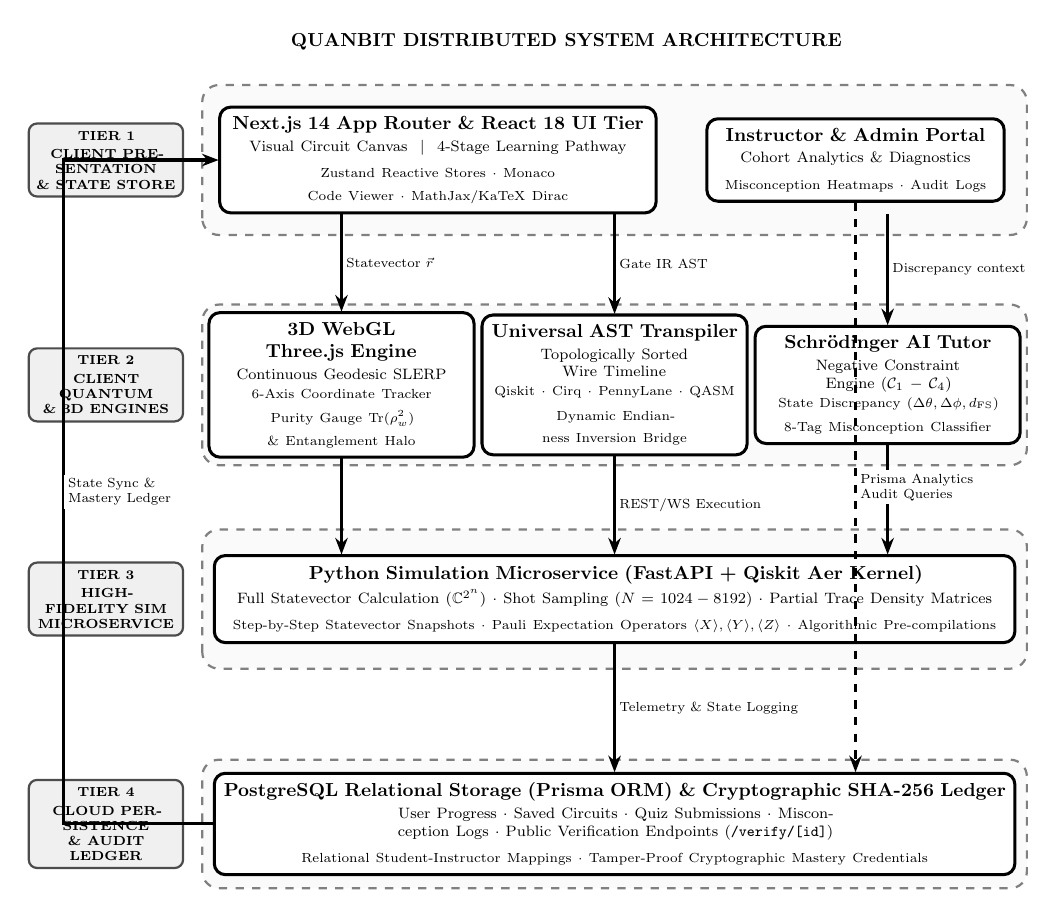
\begin{tikzpicture}[
	scale=0.68, every node/.style={transform shape},
	tierbox/.style={draw=black!50, dashed, line width=0.8pt, rounded corners=6pt, fill=black!2},
	tierlabel/.style={fill=gray!12, draw=black!70, line width=0.8pt, rounded corners=3pt, font=\bfseries\scriptsize, align=center, inner sep=4pt},
	cnode/.style={draw=black, rounded corners=4pt, line width=1.1pt, align=center, fill=white, inner sep=5pt},
	arrow/.style={-{Stealth[length=6pt]}, line width=1.1pt},
	darrow/.style={-{Stealth[length=6pt]}, line width=1.1pt, dashed},
	lbl/.style={fill=white, inner sep=2pt, font=\scriptsize}
]

	% Overall Diagram Title
	\node[font=\bfseries\normalsize] at (7.0, 13.4) {QUANBIT DISTRIBUTED SYSTEM ARCHITECTURE};

	% =========================================================================
	% LEFT-SIDEBAR TIER IDENTIFIERS
	% =========================================================================
	\node[tierlabel, text width=2.6cm] at (-1.6, 11.2) {\textbf{TIER 1}\\[2pt]\scriptsize CLIENT PRESENTATION\\\& STATE STORE};
	\node[tierlabel, text width=2.6cm] at (-1.6, 7.0) {\textbf{TIER 2}\\[2pt]\scriptsize CLIENT QUANTUM\\\& 3D ENGINES};
	\node[tierlabel, text width=2.6cm] at (-1.6, 3.0) {\textbf{TIER 3}\\[2pt]\scriptsize HIGH-FIDELITY SIM\\MICROSERVICE};
	\node[tierlabel, text width=2.6cm] at (-1.6, -1.2) {\textbf{TIER 4}\\[2pt]\scriptsize CLOUD PERSISTENCE\\\& AUDIT LEDGER};

	% =========================================================================
	% TIER 1: CLIENT PRESENTATION TIER
	% =========================================================================
	\draw[tierbox] (0.2, 9.8) rectangle (15.6, 12.6);

	% Next.js Web App
	\node[cnode, text width=7.8cm] (nextapp) at (4.6, 11.2) {
		\textbf{Next.js 14 App Router \& React 18 UI Tier}\\[2pt]
		\footnotesize Visual Circuit Canvas \ \textbar\ \ 4-Stage Learning Pathway\\[2pt]
		\scriptsize Zustand Reactive Stores $\cdot$ Monaco Code Viewer $\cdot$ MathJax/KaTeX Dirac
	};

	% Admin & Instructor Portal
	\node[cnode, text width=5.2cm] (adminportal) at (12.4, 11.2) {
		\textbf{Instructor \& Admin Portal}\\[2pt]
		\footnotesize Cohort Analytics \& Diagnostics\\[2pt]
		\scriptsize Misconception Heatmaps $\cdot$ Audit Logs
	};

	% =========================================================================
	% TIER 2: CLIENT QUANTUM & 3D ENGINES
	% =========================================================================
	\draw[tierbox] (0.2, 5.5) rectangle (15.6, 8.5);

	% 3D WebGL Bloch Sphere Engine
	\node[cnode, text width=4.6cm] (bloch3d) at (2.8, 7.0) {
		\textbf{3D WebGL Three.js Engine}\\[2pt]
		\footnotesize Continuous Geodesic SLERP\\[2pt]
		\scriptsize 6-Axis Coordinate Tracker\\[1pt]
		\scriptsize Purity Gauge $\text{Tr}(\rho_w^2)$ \& Entanglement Halo
	};

	% Universal Multi-Backend AST Transpiler
	\node[cnode, text width=4.6cm] (asttranspiler) at (7.9, 7.0) {
		\textbf{Universal AST Transpiler}\\[2pt]
		\footnotesize Topologically Sorted Wire Timeline\\[2pt]
		\scriptsize Qiskit $\cdot$ Cirq $\cdot$ PennyLane $\cdot$ QASM\\[1pt]
		\scriptsize Dynamic Endianness Inversion Bridge
	};

	% Schr{\"o}dinger AI Socratic Tutor
	\node[cnode, text width=4.6cm] (socratictutor) at (13.0, 7.0) {
		\textbf{Schr{\"o}dinger AI Tutor}\\[2pt]
		\footnotesize Negative Constraint Engine ($\mathcal{C}_1-\mathcal{C}_4$)\\[2pt]
		\scriptsize State Discrepancy ($\Delta\theta, \Delta\phi, d_{\text{FS}}$)\\[1pt]
		\scriptsize 8-Tag Misconception Classifier
	};

	% =========================================================================
	% TIER 3: HIGH-FIDELITY SIMULATION MICROSERVICE
	% =========================================================================
	\draw[tierbox] (0.2, 1.7) rectangle (15.6, 4.3);

	% FastAPI Python Simulation Engine
	\node[cnode, text width=14.6cm] (fastapisim) at (7.9, 3.0) {
		\textbf{Python Simulation Microservice (FastAPI + Qiskit Aer Kernel)}\\[2pt]
		\footnotesize Full Statevector Calculation ($\mathbb{C}^{2^n}$) $\cdot$ Shot Sampling ($N=1024-8192$) $\cdot$ Partial Trace Density Matrices\\[2pt]
		\scriptsize Step-by-Step Statevector Snapshots $\cdot$ Pauli Expectation Operators $\langle X \rangle, \langle Y \rangle, \langle Z \rangle$ $\cdot$ Algorithmic Pre-compilations
	};

	% =========================================================================
	% TIER 4: CLOUD PERSISTENCE & AUDIT LEDGER
	% =========================================================================
	\draw[tierbox] (0.2, -2.4) rectangle (15.6, 0.0);

	% PostgreSQL & Prisma Database
	\node[cnode, text width=14.6cm] (dbcloud) at (7.9, -1.2) {
		\textbf{PostgreSQL Relational Storage (Prisma ORM) \& Cryptographic SHA-256 Ledger}\\[2pt]
		\footnotesize User Progress $\cdot$ Saved Circuits $\cdot$ Quiz Submissions $\cdot$ Misconception Logs $\cdot$ Public Verification Endpoints (\texttt{/verify/[id]})\\[2pt]
		\scriptsize Relational Student-Instructor Mappings $\cdot$ Tamper-Proof Cryptographic Mastery Credentials
	};

	% =========================================================================
	% CONNECTIONS
	% =========================================================================

	% Next.js -> Bloch3D
	\draw[arrow] (nextapp.south -| bloch3d) -- node[lbl, right] {Statevector $\vec{r}$} (bloch3d.north);

	% Next.js -> AST Transpiler
	\draw[arrow] (nextapp.south -| asttranspiler) -- node[lbl, right] {Gate IR AST} (asttranspiler.north);

	% Next.js -> Socratic Tutor
	\draw[arrow] (nextapp.south -| socratictutor) -- node[lbl, right] {Discrepancy context} (socratictutor.north);

	% Bloch3D -> FastAPI Sim
	\draw[arrow] (bloch3d.south) -- (fastapisim.north -| bloch3d);

	% AST Transpiler -> FastAPI Sim
	\draw[arrow] (asttranspiler.south) -- node[lbl, right] {REST/WS Execution} (fastapisim.north -| asttranspiler);

	% Socratic Tutor -> FastAPI Sim
	\draw[arrow] (socratictutor.south) -- (fastapisim.north -| socratictutor);

	% Admin -> DB
	\draw[darrow] (adminportal.south) -- node[lbl, right, align=left] {Prisma Analytics\\Audit Queries} (dbcloud.north -| adminportal);

	% FastAPI Sim -> DB
	\draw[arrow] (fastapisim.south) -- node[lbl, right] {Telemetry \& State Logging} (dbcloud.north -| fastapisim);

	% DB -> Next.js Return Loop (Cleanly routed with inner label)
	\draw[arrow] (dbcloud.west) -- ++(-2.8, 0) |- node[lbl, right, pos=0.25, align=left] {State Sync \&\\Mastery Ledger} (nextapp.west);

\end{tikzpicture}
\end{singlespace}
\caption{QuanBit Four-Tier Distributed System Architecture Diagram}
\label{fig:architecture}
\end{figure}

\subsection{Detailed Tier Specifications}
\begin{itemize}
	\item \textbf{Tier 1: Client Presentation Tier:}
	\begin{itemize}
		\item \textit{Next.js 14 App Router \& React 18:} Fully typed in TypeScript. Manages routing across the visual circuit workbench (\texttt{/simulator}), the 3D Bloch sphere explorer (\texttt{/bloch-sphere}), the 4-Stage Learning Pathway (\texttt{/learn}), the coding challenge arena (\texttt{/practice}), and the certificate verification engine (\texttt{/verify/[id]}).
		\item \textit{Zustand Reactive State Stores:} Provides high-performance, atomic client state management (\texttt{state-store.ts}), isolating 60 FPS drag-and-drop wire reordering and timeline scrubbing from asynchronous backend calls.
		\item \textit{Monaco Code Editor \& KaTeX Dirac Visualizer:} Displays live, synchronized syntax-highlighted code panels and mathematical Dirac bra-ket notations.
	\end{itemize}

	\item \textbf{Tier 2: Client Quantum and 3D Visual Engines:}
	\begin{itemize}
		\item \textit{Three.js 3D Bloch Sphere Engine:} Renders an interactive 6-axis spatial coordinate sphere with real-time continuous geodesic trajectories and an automated reduced density matrix trace purity gauge ($\gamma = \text{Tr}(\rho_w^2)$).
		\item \textit{Universal AST Transpiler Engine:} Traverses the circuit Intermediate Representation (IR) along topologically sorted time slices to emit runnable IBM Qiskit, Google Cirq, Xanadu PennyLane, and OpenQASM code synchronously.
		\item \textit{Schr{\"o}dinger AI Socratic Tutoring Engine:} Evaluates statevector fidelity ($F$), Fubini-Study distance ($d_{\text{FS}}$), and spherical coordinate errors ($\Delta\theta, \Delta\phi$), executing prompt cascades governed by negative constraints ($\mathcal{C}_1-\mathcal{C}_4$).
	\end{itemize}

	\item \textbf{Tier 3: Python High-Fidelity Simulation Microservice:}
	\begin{itemize}
		\item \textit{FastAPI + Qiskit Aer Engine (`services/quantum-sim`):} Handles high-dimensional statevector operations ($\mathbb{C}^{2^n}$ for $n \le 16$), partial trace density operator calculations, and shot-based quantum measurement sampling ($N=1024$ to $8192$ shots).
		\item \textit{Step-by-Step Intermediate State Inspector:} Generates discrete statevector snapshots at each time slice $\tau$ along the circuit timeline, enabling timeline scrubbing.
	\end{itemize}

	\item \textbf{Tier 4: Cloud Persistence and Verification Ledger:}
	\begin{itemize}
		\item \textit{PostgreSQL via Prisma ORM:} Relational data store persisting student profiles, module progress, quiz logs, saved circuits, practice submissions, and cohort misconception telemetry.
		\item \textit{SHA-256 Public Certificate Ledger:} Stores cryptographically minted mastery credentials accessible to employers and institutions via public REST endpoints (\texttt{/verify/[id]}).
	\end{itemize}
\end{itemize}

\newpage

% =========================================================================
% Section 3: 3D Statevector Mechanics & Density Matrix Diagnostics
% =========================================================================
\section{3D Statevector Mechanics and Density Matrix Diagnostics}

\subsection{Mathematical Parameterization of the 6-Axis Bloch Sphere}
Any pure single-qubit quantum state $|\psi\rangle \in \mathcal{H}_2$ can be parameterized up to an unobservable global phase factor $e^{i\alpha}$ as:
\begin{equation}
|\psi\rangle = \cos\left(\frac{\theta}{2}\right)|0\rangle + e^{i\phi}\sin\left(\frac{\theta}{2}\right)|1\rangle
\end{equation}
where $\theta \in [0, \pi]$ represents the polar angle and $\phi \in [0, 2\pi)$ represents the azimuthal relative phase angle. The corresponding Cartesian coordinates on the unit sphere $\mathcal{S}^2 \subset \mathbb{R}^3$ are given by:
\begin{equation}
\vec{r} = \begin{bmatrix} x \\ y \\ z \end{bmatrix} = \begin{bmatrix} \sin\theta\cos\phi \\ \sin\theta\sin\phi \\ \cos\theta \end{bmatrix}
\end{equation}

To eliminate spatial disorientation, QuanBit projects six spatial HTML poles anchored dynamically in WebGL 3D space:
\begin{itemize}
	\item \textbf{$+Z$ Pole ($|0\rangle$):} Coordinates $(0, 1.55, 0)$ --- Computational ground state.
	\item \textbf{$-Z$ Pole ($|1\rangle$):} Coordinates $(0, -1.55, 0)$ --- Computational excited state.
	\item \textbf{$+X$ Pole ($|+\rangle$):} Coordinates $(1.55, 0, 0)$ --- Symmetric superposition state $\frac{|0\rangle+|1\rangle}{\sqrt{2}}$.
	\item \textbf{$-X$ Pole ($|-\rangle$):} Coordinates $(-1.55, 0, 0)$ --- Anti-symmetric superposition state $\frac{|0\rangle-|1\rangle}{\sqrt{2}}$.
	\item \textbf{$+Y$ Pole ($|i\rangle$):} Coordinates $(0, 0, 1.55)$ --- Complex circular phase state $\frac{|0\rangle+i|1\rangle}{\sqrt{2}}$.
	\item \textbf{$-Y$ Pole ($|-i\rangle$):} Coordinates $(0, 0, -1.55)$ --- Conjugate phase state $\frac{|0\rangle-i|1\rangle}{\sqrt{2}}$.
\end{itemize}

\subsection{Continuous Geodesic Trajectories via Spherical Linear Interpolation (SLERP)}
When a single-qubit unitary gate $U(\beta, \vec{n}) = \exp(-i \frac{\beta}{2} \vec{n} \cdot \vec{\sigma})$ is placed on the circuit canvas, the statevector undergoes a spatial rotation of angle $\beta$ about unit axis $\vec{n}$. Rather than snapping abruptly, QuanBit's rendering pipeline computes continuous geodesic arcs across the sphere's surface using Spherical Linear Interpolation (SLERP):
\begin{equation}
\vec{r}(t) = \frac{\sin((1-t)\Omega)}{\sin\Omega}\vec{r}_0 + \frac{\sin(t\Omega)}{\sin\Omega}\vec{r}_1, \quad \text{where } \Omega = \arccos(\vec{r}_0 \cdot \vec{r}_1)
\end{equation}
for normalized time parameter $t \in [0, 1]$. This fluid animation allows students to physically perceive phase rotation (e.g., observing the $T$-gate execute a $45^\circ$ rotation along the equatorial plane about the $Z$-axis).

\subsection{Reduced Density Matrix Formulation and Trace Purity Collapse}
For an $n$-qubit register in global pure state $|\psi\rangle \in \mathbb{C}^{2^n}$, the global density operator is $\rho = |\psi\rangle\langle\psi|$. To evaluate the local physical state of an individual target wire $w \in [0, n-1]$, the complementary wires $\bar{w} = \{0, \dots, n-1\} \setminus \{w\}$ are traced out via the \textit{partial trace}:
\begin{equation}
\rho_w = \text{Tr}_{\bar{w}}(\rho) = \begin{bmatrix} \rho_{00} & \rho_{01} \\ \rho_{10} & \rho_{11} \end{bmatrix}
\end{equation}
The local Bloch vector coordinates $\vec{r}_w = (x_w, y_w, z_w)$ are derived directly from Pauli operator expectation values:
\begin{equation}
x_w = \text{Tr}(\rho_w \sigma_x) = 2\,\text{Re}(\rho_{01}), \quad y_w = \text{Tr}(\rho_w \sigma_y) = -2\,\text{Im}(\rho_{01}), \quad z_w = \text{Tr}(\rho_w \sigma_z) = \rho_{00} - \rho_{11}
\end{equation}
The degree of quantum mixing and entanglement is quantified by the \textbf{trace purity} $\gamma$:
\begin{equation}
\gamma = \text{Tr}(\rho_w^2) = \rho_{00}^2 + \rho_{11}^2 + 2|\rho_{01}|^2 \in \left[ \frac{1}{2}, 1.0 \right]
\end{equation}
The physical magnitude of the Bloch vector inside the unit ball relates directly to purity:
\begin{equation}
|\vec{r}_w| = \sqrt{x_w^2 + y_w^2 + z_w^2} = \sqrt{2\gamma - 1}
\end{equation}

\noindent\textbf{Theorem 1 (Analytical Proof of Purity Collapse in Bell States):} \textit{For a two-qubit register in the maximally entangled Bell state $|\Phi^+\rangle = \frac{|00\rangle + |11\rangle}{\sqrt{2}}$, the reduced density operator of qubit 0 yields a trace purity of exactly $\gamma = 0.5$, causing the Bloch vector radius to collapse to zero.}

\vspace{0.2cm}
\begin{singlespace}
\noindent\textit{Proof.} The global bipartite density operator is:
$$\rho = |\Phi^+\rangle\langle\Phi^+| = \frac{1}{2}\begin{bmatrix} 1 & 0 & 0 & 1 \\ 0 & 0 & 0 & 0 \\ 0 & 0 & 0 & 0 \\ 1 & 0 & 0 & 1 \end{bmatrix}$$
Tracing over qubit 1 using the standard computational basis $\{|0\rangle, |1\rangle\}$:
$$\rho_0 = \text{Tr}_1(\rho) = \sum_{k \in \{0, 1\}} (I \otimes \langle k|)\rho(I \otimes |k\rangle) = \frac{1}{2}(|0\rangle\langle 0| + |1\rangle\langle 1|) = \frac{1}{2}I_2 = \begin{bmatrix} 0.5 & 0 \\ 0 & 0.5 \end{bmatrix}$$
Evaluating trace purity $\gamma$:
$$\gamma = \text{Tr}(\rho_0^2) = \text{Tr}\left( \begin{bmatrix} 0.25 & 0 \\ 0 & 0.25 \end{bmatrix} \right) = 0.25 + 0.25 = 0.5$$
Calculating the corresponding Bloch vector magnitude:
$$|\vec{r}_0| = \sqrt{2\gamma - 1} = \sqrt{2(0.5) - 1} = \sqrt{0} = 0 \quad \blacksquare$$
\end{singlespace}
\vspace{0.2cm}

\subsection{Visual Radial Contraction and Diagnostic Entanglement Halo}
When $\gamma < 0.999$, QuanBit's WebGL renderer initiates two visual feedback mechanisms:
\begin{enumerate}[label=\textbf{\arabic*.}]
	\item \textbf{Radial Vector Contraction:} The 3D arrow collapses toward the coordinate center $\vec{0} = (0,0,0)$ proportionally to $|\vec{r}_w| = \sqrt{2\gamma - 1}$.
	\item \textbf{Amber Entanglement Halo:} The standard vector head transitions into an amber pulsating spherical aura ($r = 0.35$). An interactive tooltip alerts the learner: \textit{``Qubit $w$ is in a maximally mixed statistical state ($\gamma=0.500$). Bipartite entanglement with complementary qubits renders single-qubit Bloch coordinates physically undefined.''}
\end{enumerate}

\newpage

% =========================================================================
% Section 4: Universal Multi-Backend AST Transpilation Engine
% =========================================================================
\section{Universal Multi-Backend AST Transpilation Engine}

\subsection{Intermediate Representation (IR) Abstract Syntax Tree Specification}
To enable framework-agnostic circuit manipulation, QuanBit abstracts visual circuit layouts into a formal Intermediate Representation (IR) Abstract Syntax Tree:
\begin{equation}
\mathcal{C}_{\text{AST}} = \left( n_{\text{qubits}}, \{ g_k = (\tau_k, \text{type}_k, \mathbf{q}_k, \mathbf{\theta}_k) \}_{k=1}^M \right)
\end{equation}
where $\tau_k \in \mathbb{N}$ denotes the discrete execution time slice (topological step), $\text{type}_k \in \mathcal{G}$ is the quantum operator from the universal gate set:
\begin{equation}
\mathcal{G} = \{ H, X, Y, Z, S, T, R_x, R_y, R_z, CX, CZ, SWAP, M \}
\end{equation}
$\mathbf{q}_k = (q_{\text{control}}, q_{\text{target}})$ defines the wire coordinates, and $\mathbf{\theta}_k \in [0, 2\pi)$ specifies continuous rotation angles for parameterized phase gates.

\subsection{Bidirectional Code Generation Rules Across Target SDKs}
The compiler traverses the IR AST and emits syntactically verified code across four industrial target SDKs simultaneously, as defined in Table~\ref{tab:transpile_rules}.

\begin{table}[htbp]
\centering
\caption{Universal AST Code Emission Mapping Across Quantum Frameworks}
\label{tab:transpile_rules}
\resizebox{\textwidth}{!}{%
\begin{tabular}{@{}lllll@{}}
\toprule
\textbf{Operator} & \textbf{IBM Qiskit} & \textbf{Google Cirq} & \textbf{Xanadu PennyLane} & \textbf{OpenQASM (2.0/3.0)} \\
\midrule
Hadamard ($H$) & \texttt{qc.h(q)} & \texttt{cirq.H(q)} & \texttt{qml.Hadamard(wires=q)} & \texttt{h q[q];} \\[3pt]
Pauli-X ($X$) & \texttt{qc.x(q)} & \texttt{cirq.X(q)} & \texttt{qml.PauliX(wires=q)} & \texttt{x q[q];} \\[3pt]
Pauli-Y ($Y$) & \texttt{qc.y(q)} & \texttt{cirq.Y(q)} & \texttt{qml.PauliY(wires=q)} & \texttt{y q[q];} \\[3pt]
Pauli-Z ($Z$) & \texttt{qc.z(q)} & \texttt{cirq.Z(q)} & \texttt{qml.PauliZ(wires=q)} & \texttt{z q[q];} \\[3pt]
Phase ($S$) & \texttt{qc.s(q)} & \texttt{cirq.S(q)} & \texttt{qml.S(wires=q)} & \texttt{s q[q];} \\[3pt]
$\pi/8$ Gate ($T$) & \texttt{qc.t(q)} & \texttt{cirq.T(q)} & \texttt{qml.T(wires=q)} & \texttt{t q[q];} \\[3pt]
Rotation ($R_x(\theta)$) & \texttt{qc.rx(th, q)} & \texttt{cirq.rx(th)(q)} & \texttt{qml.RX(th, wires=q)} & \texttt{rx(th) q[q];} \\[3pt]
Controlled-NOT & \texttt{qc.cx(c, t)} & \texttt{cirq.CNOT(c, t)} & \texttt{qml.CNOT(wires=[c,t])} & \texttt{cx q[c], q[t];} \\[3pt]
Controlled-Z & \texttt{qc.cz(c, t)} & \texttt{cirq.CZ(c, t)} & \texttt{qml.CZ(wires=[c,t])} & \texttt{cz q[c], q[t];} \\[3pt]
SWAP Gate & \texttt{qc.swap(a, b)} & \texttt{cirq.SWAP(a, b)} & \texttt{qml.SWAP(wires=[a,b])} & \texttt{swap q[a], q[b];} \\[3pt]
Measurement & \texttt{qc.measure(q, c)} & \texttt{cirq.measure(q)} & \texttt{qml.sample(wires=q)} & \texttt{measure q[q] -> c[c];} \\
\bottomrule
\end{tabular}%
}
\end{table}

\subsection{Register Endianness Normalization Bridge}
A pervasive source of confusion among novice programmers is register endianness:
\begin{itemize}
	\item \textbf{Little-Endian (IBM Qiskit):} Wire 0 represents the least significant bit ($|q_{n-1} \dots q_1 q_0\rangle$). For a 2-qubit register where $q_0 = |1\rangle$ and $q_1 = |0\rangle$, Qiskit indexes the state as basis string \texttt{"01"} (integer 1).
	\item \textbf{Big-Endian (Google Cirq, PennyLane, KaTeX Dirac):} Wire 0 represents the most significant bit ($|q_0 q_1 \dots q_{n-1}\rangle$). The same physical configuration produces basis string \texttt{"10"} (integer 2).
\end{itemize}
QuanBit's transpiler normalizes this transformation in real time. It renders side-by-side terminal tabs and visual probability distributions with bidirectional annotations, allowing learners to understand why identical quantum states yield inverted binary labels across SDK outputs without silent indexing bugs.

\newpage

% =========================================================================
% Section 5: Schr{\"o}dinger AI Socratic Guidance Architecture
% =========================================================================
\section{Schr{\"o}dinger AI: Socratic Guidance Architecture}

\subsection{Formal Negative Constraint Specification}
To eliminate passive cognitive offloading, QuanBit introduces \textbf{Schr{\"o}dinger AI}, an intelligent pedagogical tutoring agent governed by a formal negative-constraint prompt grammar $\mathcal{C} = \{\mathcal{C}_1, \mathcal{C}_2, \mathcal{C}_3, \mathcal{C}_4\}$:
\begin{equation}
\label{eq:ai_rules}
\begin{aligned}
\mathcal{C}_1 &: \text{Forbidden}(\text{Direct Gate Names } g \in \mathcal{G}) \\
\mathcal{C}_2 &: \text{Forbidden}(\text{Explicit Wire Coordinates } q_k) \\
\mathcal{C}_3 &: \text{Mandatory}(\text{State Discrepancy Analysis: } \Delta\theta, \Delta\phi, \Delta P) \\
\mathcal{C}_4 &: \text{Mandatory}(\text{Targeted Socratic Query Prompting})
\end{aligned}
\end{equation}
Specifically, $\mathcal{C}_1$ forbids uttering operator names $\{H, X, Y, Z, S, T, CX, CZ\}$, $\mathcal{C}_2$ forbids coordinate commands (e.g., ``place gate on wire 0''), $\mathcal{C}_3$ grounds guidance in physical statevector discrepancies, and $\mathcal{C}_4$ prompts the learner to independently deduce the necessary unitary operator.

\begin{figure}[htbp]
\centering
\begin{singlespace}
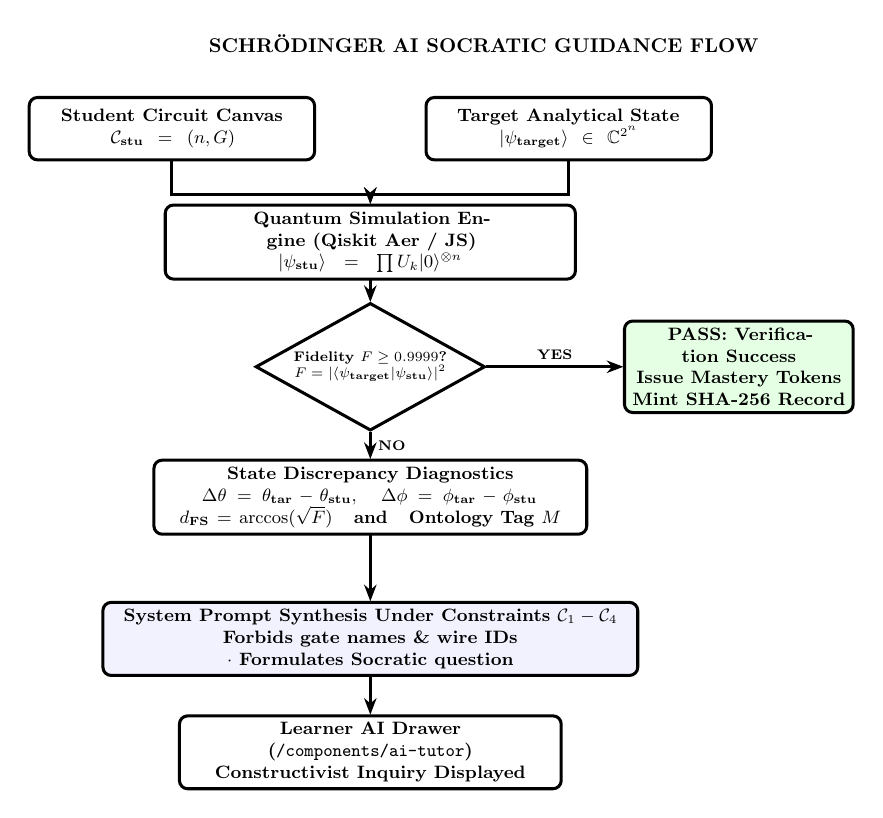
\begin{tikzpicture}[
	scale=0.72, every node/.style={transform shape},
	pbox/.style={draw=black, line width=1.1pt, rounded corners=3pt, fill=white, font=\bfseries\small, align=center, minimum height=1.1cm},
	msg/.style={-{Stealth[length=6pt]}, line width=1.1pt},
	decision/.style={diamond, draw=black, line width=1.1pt, fill=white, font=\bfseries\scriptsize, align=center, inner sep=2pt, aspect=1.8}
]
	% Sequence Reference
	\node[font=\bfseries\normalsize] at (7.0, 10.5) {SCHR{\"O}DINGER AI SOCRATIC GUIDANCE FLOW};

	% Step 1: Input Circuit
	\node[pbox, text width=4.8cm] (inputcirc) at (1.5, 9.0) {Student Circuit Canvas\\$\mathcal{C}_{\text{stu}} = (n, G)$};
	\node[pbox, text width=4.8cm] (targetstate) at (8.5, 9.0) {Target Analytical State\\$|\psi_{\text{target}}\rangle \in \mathbb{C}^{2^n}$};

	% Step 2: Simulation & Statevector
	\node[pbox, text width=7.0cm] (simengine) at (5.0, 7.0) {Quantum Simulation Engine (Qiskit Aer / JS)\\$|\psi_{\text{stu}}\rangle = \prod U_k |0\rangle^{\otimes n}$};

	% Step 3: Fidelity Judge
	\node[decision] (judge) at (5.0, 4.8) {Fidelity $F \ge 0.9999$?\\$F = |\langle\psi_{\text{target}}|\psi_{\text{stu}}\rangle|^2$};

	% Step 4: Pass / Reject
	\node[pbox, text width=3.8cm, fill=green!10] (passbox) at (11.5, 4.8) {\textbf{PASS: Verification Success}\\Issue Mastery Tokens\\Mint SHA-256 Record};
	\node[pbox, text width=7.4cm] (diagbox) at (5.0, 2.5) {State Discrepancy Diagnostics\\$\Delta\theta = \theta_{\text{tar}} - \theta_{\text{stu}}, \quad \Delta\phi = \phi_{\text{tar}} - \phi_{\text{stu}}$\\$d_{\text{FS}} = \arccos(\sqrt{F}) \quad \text{and} \quad \text{Ontology Tag } M$};

	% Step 5: Socratic Prompt Synthesis
	\node[pbox, text width=9.2cm, fill=blue!5] (socraticprompt) at (5.0, 0.0) {System Prompt Synthesis Under Constraints $\mathcal{C}_1-\mathcal{C}_4$\\Forbids gate names \& wire IDs $\cdot$ Formulates Socratic question};

	% Step 6: Output To Student Drawer
	\node[pbox, text width=6.5cm] (outputdrawer) at (5.0, -2.0) {Learner AI Drawer (\texttt{/components/ai-tutor})\\Constructivist Inquiry Displayed};

	% Connections
	\draw[msg] (inputcirc.south) -- ++(0, -0.6) -| (simengine.north);
	\draw[msg] (targetstate.south) -- ++(0, -0.6) -| (simengine.north);
	\draw[msg] (simengine.south) -- (judge.north);
	\draw[msg] (judge.east) -- node[above, font=\scriptsize\bfseries] {YES} (passbox.west);
	\draw[msg] (judge.south) -- node[right, font=\scriptsize\bfseries] {NO} (diagbox.north);
	\draw[msg] (diagbox.south) -- (socraticprompt.north);
	\draw[msg] (socraticprompt.south) -- (outputdrawer.north);

\end{tikzpicture}
\end{singlespace}
\caption{Schr{\"o}dinger AI Socratic Guidance and Verification Flow}
\label{fig:ai_flow}
\end{figure}

\subsection{Statevector Discrepancy Diagnostics}
As illustrated in Figure~\ref{fig:ai_flow}, Schr{\"o}dinger AI calculates the exact physical discrepancy between the active circuit state $|\psi_{\text{stu}}\rangle$ and target state $|\psi_{\text{target}}\rangle$:
\begin{equation}
F(|\psi_{\text{target}}\rangle, |\psi_{\text{stu}}\rangle) = |\langle \psi_{\text{target}} | \psi_{\text{stu}} \rangle|^2
\end{equation}
\begin{equation}
d_{\text{FS}}(|\psi_{\text{target}}\rangle, |\psi_{\text{stu}}\rangle) = \arccos\left(\sqrt{F}\right)
\end{equation}
\begin{equation}
\Delta\theta = \theta_{\text{target}} - \theta_{\text{stu}}, \quad \Delta\phi = \phi_{\text{target}} - \phi_{\text{stu}}
\end{equation}
Instead of instructing \textit{``Place a Hadamard gate on qubit 0''}, Schr{\"o}dinger AI detects that $\Delta\theta = \pi/2$ and $\Delta\phi = 0$ and prompts: \textit{``Notice that your statevector currently points directly toward the North Pole ($|0\rangle$). To achieve equal probability amplitudes of measuring 0 and 1 without introducing a complex phase, which unitary rotation maps the $Z$-axis onto the positive $X$-axis?''}

\subsection{Automated 8-Tag Quantum Misconception Diagnostic Ontology}
QuanBit incorporates an automated diagnostic classifier (`src/lib/ai-engine.ts`) mapping learner errors to 8 validated misconceptions:
\begin{enumerate}[label=\textbf{\arabic*.}]
	\item \texttt{SUPERPOSITION\_VS\_CLASSICAL\_PROB:} Confusing quantum probability amplitudes with classical coin-toss probabilities.
	\item \texttt{ENTANGLEMENT\_COMMUNICATION:} Believing quantum entanglement enables instantaneous faster-than-light communication.
	\item \texttt{PHASE\_KICKBACK\_MISUNDERSTANDING:} Assuming the control qubit remains completely unaffected during CNOT operations.
	\item \texttt{NO\_CLONING\_VIOLATION:} Attempting to duplicate an unknown quantum statevector.
	\item \texttt{MEASUREMENT\_COLLAPSE:} Assuming quantum superpositions persist unchanged after projective measurement.
	\item \texttt{DEUTSCH\_ORACLE\_QUERY:} Believing multiple sequential queries are required to evaluate global oracle parity.
	\item \texttt{GROVER\_AMPLITUDE\_MEAN:} Assuming the Grover oracle alone amplifies target probability without the diffusion operator.
	\item \texttt{SUPERDENSE\_BIT\_CAPACITY:} Believing two physical qubits are transmitted rather than two classical bits over one physical qubit.
\end{enumerate}

\newpage

% =========================================================================
% Section 6: Curricular Lifecycle, Algorithmic Modules & State Machine
% =========================================================================
\section{Curricular Lifecycle, Algorithmic Modules and State Machine}

\subsection{The 4-Stage Pedagogical Scaffolding Progression}
Every quantum algorithm module follows a structured 4-stage instructional progression grounded in Cognitive Load Theory and Bloom's Revised Taxonomy:
\begin{itemize}
	\item \textbf{Stage 1: Dual Intuition \& Dirac Mathematical Formulation:} The learner explores the algorithm via a dual-explanation toggle: \textit{Intuitive Mode} (everyday analogies, optical beam splitters, coin flips) vs. \textit{Technical Mode} (Dirac statevectors, bra-ket notation, and unitary matrices).
	\item \textbf{Stage 2: 3D Geodesic Sandbox Simulation:} An interactive Three.js sandbox where students drag gates and observe real-time geodesic statevector sweeps, relative phase shifts, and entanglement purity collapse.
	\item \textbf{Stage 3: Milestone-Driven ``Build-It'' Circuit Synthesis:} Students must construct the complete quantum circuit from scratch against analytical test cases, receiving real-time validation from Schr{\"o}dinger AI.
	\item \textbf{Stage 4: Adaptive Mastery Testing:} An assessment quiz evaluating conceptual retention and algorithmic problem-solving. Achieving $\ge 75\%$ unlocks the next curriculum module and issues a cryptographic mastery credential.
\end{itemize}

\subsection{State Machine Specifications}
The operational lifecycle of a student progression session transitions through five distinct states, as modeled in Figure~\ref{fig:state_machine}.

\begin{figure}[htbp]
\centering
\begin{singlespace}
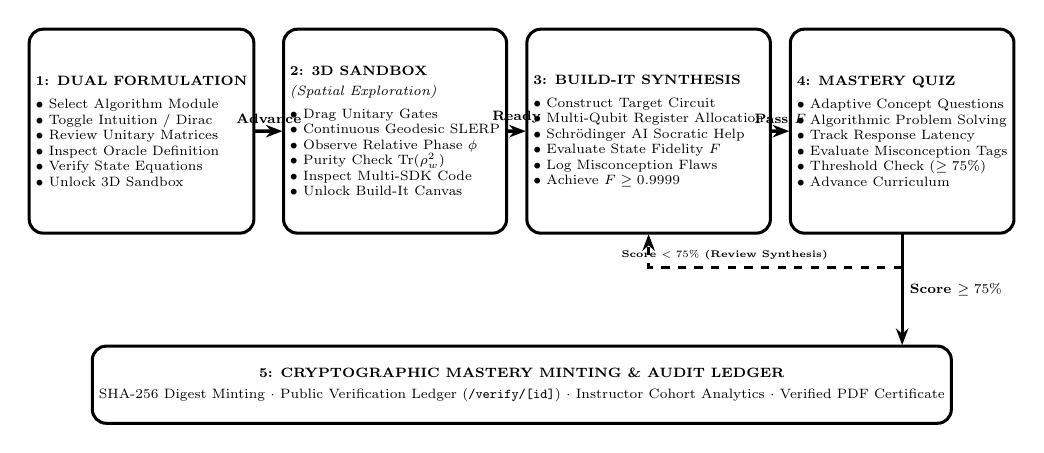
\begin{tikzpicture}[
	scale=0.70, every node/.style={transform shape},
	statebox/.style={draw=black, line width=1.1pt, rounded corners=5pt, align=left, font=\scriptsize, fill=white, minimum width=3.1cm, minimum height=3.7cm},
	trans/.style={-{Stealth[length=6pt]}, line width=1.2pt, draw=black}
]
	% State 1: Stage 1
	\node[statebox] (s1) at (0, 6.0) {
		\textbf{1: DUAL FORMULATION}\\[4pt]
		$\bullet$ Select Algorithm Module\\
		$\bullet$ Toggle Intuition / Dirac\\
		$\bullet$ Review Unitary Matrices\\
		$\bullet$ Inspect Oracle Definition\\
		$\bullet$ Verify State Equations\\
		$\bullet$ Unlock 3D Sandbox
	};

	% State 2: Stage 2
	\node[statebox, minimum width=3.4cm] (s2) at (4.6, 6.0) {
		\textbf{2: 3D SANDBOX}\\[2pt]
		\scriptsize\textit{(Spatial Exploration)}\\[4pt]
		$\bullet$ Drag Unitary Gates\\
		$\bullet$ Continuous Geodesic SLERP\\
		$\bullet$ Observe Relative Phase $\phi$\\
		$\bullet$ Purity Check $\text{Tr}(\rho_w^2)$\\
		$\bullet$ Inspect Multi-SDK Code\\
		$\bullet$ Unlock Build-It Canvas
	};

	% State 3: Stage 3
	\node[statebox] (s3) at (9.2, 6.0) {
		\textbf{3: BUILD-IT SYNTHESIS}\\[4pt]
		$\bullet$ Construct Target Circuit\\
		$\bullet$ Multi-Qubit Register Allocation\\
		$\bullet$ Schr{\"o}dinger AI Socratic Help\\
		$\bullet$ Evaluate State Fidelity $F$\\
		$\bullet$ Log Misconception Flaws\\
		$\bullet$ Achieve $F \ge 0.9999$
	};

	% State 4: Stage 4
	\node[statebox] (s4) at (13.8, 6.0) {
		\textbf{4: MASTERY QUIZ}\\[4pt]
		$\bullet$ Adaptive Concept Questions\\
		$\bullet$ Algorithmic Problem Solving\\
		$\bullet$ Track Response Latency\\
		$\bullet$ Evaluate Misconception Tags\\
		$\bullet$ Threshold Check ($\ge 75\%$)\\
		$\bullet$ Advance Curriculum
	};

	% State 5: Credentialing
	\node[draw=black, line width=1.1pt, rounded corners=5pt, align=center, font=\scriptsize, minimum width=15.4cm, minimum height=1.4cm, fill=white] (s5) at (6.9, 1.4) {
		\textbf{5: CRYPTOGRAPHIC MASTERY MINTING \& AUDIT LEDGER}\\[3pt]
		SHA-256 Digest Minting $\cdot$ Public Verification Ledger (\texttt{/verify/[id]}) $\cdot$ Instructor Cohort Analytics $\cdot$ Verified PDF Certificate
	};

	% Forward Transitions
	\draw[trans] (s1) -- node[above, font=\scriptsize\bfseries] {Advance} (s2);
	\draw[trans] (s2) -- node[above, font=\scriptsize\bfseries] {Ready} (s3);
	\draw[trans] (s3) -- node[above, font=\scriptsize\bfseries] {Pass $F$} (s4);

	% Downward Transition to Credentialing
	\draw[trans] (s4.south) -- node[right, font=\scriptsize\bfseries] {Score $\ge 75\%$} (s4.south |- s5.north);

	% Re-try loop from State 4 back to State 3
	\draw[trans, dashed] (s4.south) -- ++(0,-0.6) -| node[pos=0.35, above, font=\tiny\bfseries] {Score $< 75\%$ (Review Synthesis)} (s3.south);

\end{tikzpicture}
\end{singlespace}
\caption{Curricular Learning Lifecycle and Mastery Verification State Machine}
\label{fig:state_machine}
\end{figure}

\subsection{Curricular Algorithm Formulations}
QuanBit provides fully implemented, interactive instructional modules for four foundational quantum algorithms:
\begin{enumerate}[label=\textbf{\arabic*.}]
	\item \textbf{Deutsch-Jozsa Algorithm:} Evaluates whether an unknown Boolean oracle function $f: \{0,1\}^n \to \{0,1\}$ is constant or balanced in a single quantum evaluation. Initializing to $|0\rangle^{\otimes n}|1\rangle$ and applying Hadamard transformations:
	$$|\psi_1\rangle = \frac{1}{\sqrt{2^n}}\sum_{x=0}^{2^n-1}|x\rangle \otimes |-\rangle$$
	Applying oracle $U_f$ exploits phase kickback:
	$$|\psi_2\rangle = \frac{1}{\sqrt{2^n}}\sum_{x=0}^{2^n-1}(-1)^{f(x)}|x\rangle \otimes |-\rangle$$
	A final Hadamard layer yields measurement amplitude $C_0 = \frac{1}{2^n}\sum_{x=0}^{2^n-1}(-1)^{f(x)}$, measuring $|0\rangle^{\otimes n}$ with probability 1 if constant, and 0 if balanced.

	\item \textbf{Grover's Quantum Search Algorithm:} Locates a marked item $\omega$ in an unsorted database of $N=2^n$ items in $O(\sqrt{N})$ queries. Each Grover iteration applies the phase oracle $U_\omega = I - 2|\omega\rangle\langle\omega|$ followed by the diffusion operator $U_s = 2|s\rangle\langle s| - I$, where $|s\rangle = \frac{1}{\sqrt{N}}\sum_{x=0}^{N-1}|x\rangle$. The optimal iteration count is derived analytically as:
	$$R \approx \left\lfloor \frac{\pi}{4}\sqrt{N} \right\rfloor$$

	\item \textbf{Quantum Teleportation Protocol:} Teleports an unknown state $|\psi\rangle = \alpha|0\rangle + \beta|1\rangle$ using two classical bits and one pre-shared Bell pair $|\Phi^+\rangle = \frac{|00\rangle+|11\rangle}{\sqrt{2}}$. Alice executes a CNOT and Hadamard before measuring outcomes $(M_1, M_2) \in \{0,1\}^2$. Bob recovers the state by applying conditional unitary Pauli corrections:
	$$|\psi_{\text{out}}\rangle = X^{M_2} Z^{M_1} |\psi_{\text{received}}\rangle = \alpha|0\rangle + \beta|1\rangle$$

	\item \textbf{Superdense Coding Protocol:} Transmits two classical bits $(b_1, b_2) \in \{0,1\}^2$ through the physical manipulation and transmission of a single qubit. Alice applies one of $\{I, X, Z, XZ\}$ to her entangled qubit, steering the global state into one of four orthogonal Bell states:
	$$00 \to |\Phi^+\rangle, \quad 01 \to |\Psi^+\rangle, \quad 10 \to |\Phi^-\rangle, \quad 11 \to |\Psi^-\rangle$$
	Bob decodes with a CNOT and Hadamard gate, measuring $(b_1, b_2)$ deterministically.
\end{enumerate}

\newpage

% =========================================================================
% Section 7: Extended Platform Workflows & Ecosystem
% =========================================================================
\section{Extended Platform Workflows and Ecosystem}

\subsection{LeetCode-Style Quantum Practice Arena}
QuanBit features an integrated practice arena (`src/app/practice`) containing 40+ curated coding challenges organized across three difficulty tiers (Beginner, Intermediate, Advanced). Each problem specifies:
\begin{itemize}
	\item \textbf{Analytical Problem Objective:} Clear mathematical goal (e.g., ``Synthesize a Greenberger-Horne-Zeilinger (GHZ) state with minimal gate depth'').
	\item \textbf{Automated Test Suite:} The submission is simulated against target statevectors and measured against state fidelity threshold $F \ge 0.9999$ and gate count limits.
	\item \textbf{Instant Execution Feedback:} Displays circuit diagrams, target vs. actual state amplitudes, and Socratic hints if tests fail.
\end{itemize}

\subsection{Cryptographically Verifiable SHA-256 Public Certificate Ledger}
Upon completing all module milestones and achieving $\ge 75\%$ on the Stage 4 mastery quiz, the student is awarded a Certificate of Quantum Mastery (`src/components/certificate/QuantumCertificateModal.tsx`):
\begin{itemize}
	\item \textbf{Cryptographic Minting:} The certificate ID is synthesized via a deterministic SHA-256 hash digest:
	$$\mathcal{S} = \text{SHA-256}(\text{ID}_{\text{student}} \parallel \text{ModuleSlug} \parallel \text{Timestamp} \parallel K_{\text{private}})$$
	\item \textbf{Public Verification Endpoint:} Any prospective employer or university can verify the credential's authenticity in sub-seconds via the public route:
	$$\texttt{https://quanbit.edu/verify/\{credentialId\}}$$
	The portal displays the learner's name, module title, issuance timestamp, mastery score, and cryptographic signature hash.
\end{itemize}

\subsection{Instructor Analytics & Cohort Misconception Telemetry}
Academic educators access a dedicated institutional portal (`src/app/instructor` and `src/app/admin`) providing cohort governance:
\begin{itemize}
	\item \textbf{Cohort Progress Tracking:} Real-time visualization of student completion rates across modules, average time-to-solve, and quiz score distributions.
	\item \textbf{Real-Time Misconception Heatmaps:} Visualizes the frequency of the 8 diagnostic flaw tags across class cohorts, identifying specific conceptual hurdles (e.g., identifying that 42\% of students exhibit \texttt{PHASE\_KICKBACK\_MISUNDERSTANDING}) and enabling targeted in-class remediation.
\end{itemize}

\subsection{Universal Multilingual Support & WCAG 2.1 AA Accessibility}
QuanBit is engineered to ensure universal accessibility for global learners:
\begin{itemize}
	\item \textbf{Multilingual Localization:} Full UI translation and instructional text support across 9 languages (English, Hindi, Spanish, French, German, Tamil, Telugu, Japanese, Simplified Chinese) managed via `src/lib/i18n.ts`.
	\item \textbf{Keyboard-First Wire Navigation:} Full keyboard access for the circuit builder canvas, enabling students to place, move, and configure gates using standard hotkeys (\texttt{H}, \texttt{X}, \texttt{Y}, \texttt{Z}, \texttt{S}, \texttt{T}, \texttt{C}, \texttt{W}).
	\item \textbf{High-Contrast \& Reduced Motion Modes:} Conforms strictly with WCAG 2.1 AA standards, supporting high-contrast color palettes and disabling WebGL animation loops for motion-sensitive learners.
\end{itemize}

\newpage

% =========================================================================
% Section 8: Functional Requirements Specification
% =========================================================================
\section{Functional Requirements Specification}

Table~\ref{tab:functional_requirements} details the core functional requirements governing the QuanBit quantum pedagogical platform and multi-backend simulator.

\begingroup
\small
\setlength{\tabcolsep}{4pt}
\begin{longtable}{@{}p{2.1cm}p{3.2cm}p{9.8cm}@{}}
\caption{QuanBit Functional Requirements Specification} \label{tab:functional_requirements} \\
\toprule
\textbf{Req. ID} & \textbf{Feature Area} & \textbf{Functional Specification} \\
\midrule
\endfirsthead
\toprule
\textbf{Req. ID} & \textbf{Feature Area} & \textbf{Functional Specification} \\
\midrule
\endhead
\bottomrule
\endfoot
\textbf{FR-BLO-01} & 3D Bloch Rendering & The system shall render an interactive 6-axis WebGL Three.js Bloch sphere with spatial HTML labels for poles $|0\rangle, |1\rangle, |+\rangle, |-\rangle, |i\rangle, |-i\rangle$. \\
\textbf{FR-BLO-02} & Geodesic Trajectories & The visualizer shall compute continuous geodesic rotations via Spherical Linear Interpolation (SLERP) upon unitary gate application. \\
\textbf{FR-BLO-03} & Purity Gauge & The system shall compute reduced density matrix trace purity $\gamma = \text{Tr}(\rho_w^2)$ and contract the Bloch vector proportionally to $|\vec{r}_w| = \sqrt{2\gamma - 1}$. \\
\textbf{FR-BLO-04} & Entanglement Halo & If $\gamma < 0.999$, the renderer shall display an amber pulsating halo and an alert indicating that single-qubit Bloch coordinates are physically undefined. \\
\textbf{FR-SIM-01} & Client Circuit Canvas & The user shall construct circuits up to 5 qubits with sub-16 ms latency using single- and two-qubit gates, parameterized rotations, and measurements. \\
\textbf{FR-SIM-02} & High-Fidelity Simulation & The Python FastAPI microservice shall evaluate exact statevectors ($\mathbb{C}^{2^n}$), shot sampling ($N=1024-8192$), and Pauli expectation values $\langle X \rangle, \langle Y \rangle, \langle Z \rangle$. \\
\textbf{FR-SIM-03} & Step-by-Step Snapshots & The simulation engine shall record intermediate statevector snapshots across all discrete time slices $\tau$ along the circuit timeline. \\
\textbf{FR-AST-01} & Multi-Target Transpiler & The AST compiler shall traverse the IR and emit syntactically verified code simultaneously for IBM Qiskit, Google Cirq, Xanadu PennyLane, and OpenQASM. \\
\textbf{FR-AST-02} & Endianness Normalization & The transpiler shall automatically normalize little-endian (Qiskit) vs. big-endian (Cirq/PennyLane) register ordering with annotated visual probability tabs. \\
\textbf{FR-AI-01} & Socratic Constraint System & Schr{\"o}dinger AI shall strictly enforce negative constraints $\mathcal{C}_1-\mathcal{C}_4$, forbidding direct gate disclosures and explicit wire coordinates. \\
\textbf{FR-AI-02} & Discrepancy Diagnostics & The AI engine shall evaluate state fidelity $F$, Fubini-Study distance $d_{\text{FS}}$, and spherical coordinate errors $(\Delta\theta, \Delta\phi)$ to formulate guided queries. \\
\textbf{FR-AI-03} & Misconception Ontology & The platform shall classify learner errors into 8 validated quantum computing misconception tags and log occurrences in PostgreSQL. \\
\textbf{FR-CURR-01} & 4-Stage Pathway & The platform shall enforce a 4-stage pedagogical progression (Dual Intuition/Dirac, 3D Sandbox, Build-It Synthesis, Mastery Quiz) across 4 algorithms. \\
\textbf{FR-CURR-02} & Dual Explanation Toggle & The learning module shall allow students to toggle between intuitive analogy explanations and technical Dirac mathematical formulations. \\
\textbf{FR-PRAC-01} & Practice Arena & The platform shall provide 40+ LeetCode-style quantum coding challenges across 3 difficulty tiers with automated fidelity verification ($F \ge 0.9999$). \\
\textbf{FR-CERT-01} & Public Credential Ledger & The system shall cryptographically mint SHA-256 certificate hashes upon module mastery ($\ge 75\%$) and provide public verification at \texttt{/verify/[id]}. \\
\textbf{FR-ADM-01} & Instructor Analytics & Educators shall access cohort heatmaps displaying student progress, submission success rates, and real-time misconception distribution graphs. \\
\textbf{FR-I18N-01} & Multilingual Localization & The system shall support dynamic language switching across 9 languages (EN, HI, ES, FR, DE, TA, TE, JA, ZH) with complete UI translations. \\
\textbf{FR-ACC-01} & Keyboard Navigation & The circuit canvas shall support full keyboard navigation and gate placement hotkeys (\texttt{H}, \texttt{X}, \texttt{Y}, \texttt{Z}, \texttt{S}, \texttt{T}, \texttt{C}, \texttt{W}) under WCAG 2.1 AA. \\
\bottomrule
\end{longtable}
\endgroup

\newpage

% =========================================================================
% Section 9: Non-Functional Requirements Specification
% =========================================================================
\section{Non-Functional Requirements Specification}

\subsection{Performance and Latency Standards}
\begin{itemize}
	\item \textbf{Client Rendering Frame Rate (NFR-PERF-01):} The Three.js 3D Bloch sphere rendering loop and circuit canvas shall maintain a continuous 60 frames per second (FPS) with frame rendering times $< 16.6$ milliseconds on standard consumer laptops.
	\item \textbf{Local Mathematical Evaluation Latency (NFR-PERF-02):} Single- and two-qubit unitary operations for circuits up to $n=5$ qubits evaluated locally in JavaScript (`Float64Array`) shall compute in under 10 milliseconds.
	\item \textbf{Microservice Simulation Response Time (NFR-PERF-03):} High-fidelity Python simulation requests for circuits up to $n=10$ qubits executed via Qiskit Aer shall return statevector, probability, and shot data in under 250 milliseconds.
	\item \textbf{AST Transpilation Throughput (NFR-PERF-04):} Transpiling an active circuit AST into all four target SDKs (Qiskit, Cirq, PennyLane, OpenQASM) shall complete in under 5 milliseconds.
\end{itemize}

\subsection{Computational Precision and Correctness}
\begin{itemize}
	\item \textbf{Numerical Floating-Point Precision (NFR-PREC-01):} Complex statevector amplitudes, unitary matrices, and density operators shall be computed using 64-bit IEEE 754 double-precision floating-point arithmetic.
	\item \textbf{Purity Calculation Tolerance (NFR-PREC-02):} Trace purity $\gamma = \text{Tr}(\rho_w^2)$ shall be calculated with numerical tolerance $\epsilon = 10^{-6}$, ensuring pure states ($\gamma = 1.0$) and maximally mixed states ($\gamma = 0.5$) are strictly resolved without floating-point drift.
	\item \textbf{Fidelity Threshold Verification (NFR-PREC-03):} Circuit verification verdicts for Build-It synthesis and practice challenges shall enforce target state fidelity $F \ge 0.9999$.
\end{itemize}

\subsection{Security and Data Integrity}
\begin{itemize}
	\item \textbf{Cryptographic Credential Tamper-Proofing (NFR-SEC-01):} Certificate verification IDs must be deterministically signed using SHA-256 hashes generated from student identifiers, module slugs, issuance timestamps, and secure private keys.
	\item \textbf{SQL Injection and Data Validation (NFR-SEC-02):} All database transactions must execute via Prisma ORM parameterized queries, completely neutralizing SQL injection vulnerabilities.
	\item \textbf{Role-Based Access Control (NFR-SEC-03):} API routes governing instructor cohort analytics and administrative configuration must enforce JSON Web Token (JWT) session validation matching roles \texttt{STUDENT}, \texttt{EDUCATOR}, or \texttt{ADMIN}.
\end{itemize}

\subsection{Universal Accessibility and Usability}
\begin{itemize}
	\item \textbf{WCAG 2.1 AA Compliance (NFR-ACC-01):} All user interfaces, text elements, interactive canvas controls, and color palettes must strictly satisfy Web Content Accessibility Guidelines (WCAG) 2.1 Level AA standards.
	\item \textbf{Zero-Installation Accessibility (NFR-ACC-02):} The core educational platform must function seamlessly in standard modern web browsers (Chrome, Firefox, Safari, Edge) without requiring browser plugins, extensions, or local Python runtimes.
\end{itemize}

\newpage

% =========================================================================
% Section 10: Database Platform Architecture and Schema Specifications
% =========================================================================
\section{Database Platform Architecture and Schema Specifications}

\subsection{PostgreSQL Relational Persistence via Prisma ORM}
QuanBit utilizes PostgreSQL as its primary relational database management system, managed through Prisma ORM. The relational schema is structured to support multi-tenant educational institutions, track fine-grained granular student progress, record misconception telemetry, and provide public certificate validation.

\subsection{Detailed Relational Entity Specifications}
\begin{enumerate}[label=\textbf{\arabic*.}, itemsep=4pt, parsep=2pt]
	\item \textbf{User Entity (\texttt{User}):}\\
	Stores authenticated user profiles, credentials, institutional roles, and aggregate engagement metrics:
	\begin{itemize}[noitemsep, topsep=2pt]
		\item \texttt{id}: String (CUID, Primary Key)
		\item \texttt{name}, \texttt{email} (Unique String), \texttt{emailVerified} (DateTime)
		\item \texttt{role}: Enum (\texttt{STUDENT}, \texttt{EDUCATOR}, \texttt{ADMIN})
		\item \texttt{streakDays}: Integer (Consecutive active study days)
		\item \texttt{isPremium}: Boolean (Access flag for advanced institutional tracks)
		\item \texttt{createdAt}, \texttt{updatedAt}, \texttt{lastActiveAt} (Timestamps)
	\end{itemize}

	\item \textbf{User Progress Entity (\texttt{UserProgress}):}\\
	Tracks individual student progress across curricular algorithm modules:
	\begin{itemize}[noitemsep, topsep=2pt]
		\item \texttt{id}: String (CUID, Primary Key), \texttt{userId} (Foreign Key $\to$ \texttt{User.id})
		\item \texttt{moduleSlug}: String (e.g., \texttt{"deutsch-jozsa"}, \texttt{"grover"}, \texttt{"teleportation"})
		\item \texttt{stageReached}: Integer (1: Intuition/Math, 2: 3D Sandbox, 3: Build-It, 4: Quiz)
		\item \texttt{isCompleted}: Boolean, \texttt{masteryScore}: Float (0.0 to 100.0)
		\item \texttt{timeSpentSeconds}: Integer, \texttt{lastVisitedAt}: DateTime
		\item \textit{Constraint:} Unique compound index on \texttt{[userId, moduleSlug]}
	\end{itemize}

	\item \textbf{Quiz Attempt Entity (\texttt{QuizAttempt}):}\\
	Records question-level assessment telemetry for cognitive analysis:
	\begin{itemize}[noitemsep, topsep=2pt]
		\item \texttt{id}: String (CUID, Primary Key), \texttt{userId} (Foreign Key $\to$ \texttt{User.id})
		\item \texttt{moduleSlug}: String, \texttt{questionId}: String, \texttt{selectedAnswer}: String
		\item \texttt{isCorrect}: Boolean, \texttt{isAIAssisted}: Boolean, \texttt{timeTakenMs}: Integer
		\item \texttt{difficulty}: Enum (\texttt{BEGINNER}, \texttt{INTERMEDIATE}, \texttt{ADVANCED})
		\item \texttt{misconceptionTag}: String (Nullable diagnostic ontology tag)
	\end{itemize}

	\item \textbf{Misconception Log Entity (\texttt{MisconceptionLog}):}\\
	Maintains cumulative counts of diagnostic flaws logged by Schr{\"o}dinger AI:
	\begin{itemize}[noitemsep, topsep=2pt]
		\item \texttt{id}: String (CUID, Primary Key), \texttt{userId} (Foreign Key $\to$ \texttt{User.id})
		\item \texttt{misconceptionTag}: String (One of the 8 validated ontology tags)
		\item \texttt{occurrenceCount}: Integer, \texttt{isResolved}: Boolean, \texttt{lastFlaggedAt}: DateTime
		\textit{Constraint:} Unique compound index on \texttt{[userId, misconceptionTag]}
	\end{itemize}

	\item \textbf{Saved Circuit Entity (\texttt{SavedCircuit}):}\\
	Persists user-constructed quantum circuits in structured JSON format:
	\begin{itemize}[noitemsep, topsep=2pt]
		\item \texttt{id}: String (CUID, Primary Key), \texttt{userId} (Foreign Key $\to$ \texttt{User.id})
		\item \texttt{name}: String, \texttt{numQubits}: Integer (Default 2)
		\item \texttt{circuitJson}: JSON (Serialized AST layout, gates, parameters)
		\item \texttt{qasmCode}: String (Nullable OpenQASM export string)
	\end{itemize}

	\item \textbf{Practice Submission Entity (\texttt{PracticeSubmission}):}\\
	Logs student attempts in the LeetCode-style challenge arena:
	\begin{itemize}[noitemsep, topsep=2pt]
		\item \texttt{id}: String (CUID, Primary Key), \texttt{userId} (Foreign Key $\to$ \texttt{User.id})
		\item \texttt{moduleSlug}: String, \texttt{problemId}: String
		\item \texttt{result}: String (\texttt{"accepted"}, \texttt{"wrong\_answer"}, \texttt{"invalid\_circuit"})
		\item \texttt{isAIAssisted}: Boolean, \texttt{code}: String (Nullable circuit JSON)
	\end{itemize}

	\item \textbf{Instructor-Student Mapping Entity (\texttt{InstructorStudent}):}\\
	Enables academic educators to supervise assigned student cohorts:
	\begin{itemize}[noitemsep, topsep=2pt]
		\item \texttt{id}: String (CUID, Primary Key)
		\item \texttt{instructorId}: String (Foreign Key $\to$ \texttt{User.id})
		\item \texttt{studentId}: String (Foreign Key $\to$ \texttt{User.id})
		\item \textit{Constraint:} Unique compound index on \texttt{[instructorId, studentId]}
	\end{itemize}

	\item \textbf{AI Interaction Entity (\texttt{AIInteraction}):}\\
	Records telemetry on learner interactions with Schr{\"o}dinger AI:
	\begin{itemize}[noitemsep, topsep=2pt]
		\item \texttt{id}: String (CUID, Primary Key), \texttt{userId} (Foreign Key $\to$ \texttt{User.id})
		\item \texttt{action}: String (\texttt{"chat"}, \texttt{"generate\_circuit"}, \texttt{"debug\_circuit"}, \texttt{"diagnose\_build\_it"})
		\item \texttt{context}: String (Module slug or problem ID), \texttt{query}: String (Snippet)
	\end{itemize}
\end{enumerate}

\end{document}
